\chapter{Mécanismes de sécurité et mise en production}

\section{Protections générales}
\subsection{Durée de la session}
Par défaut, les sessions ont une durée de vie d'une heure sans activité. Elles sont supprimées automatiquement, sans tenir compte le cas échéant du cookie de session. Ce dernier est transmis en \textit{http\_only} et en mode \textit{secure}.

Si la session dure plus d'une heure\footnote{la durée par défaut de la session}, l'identifiant de session est régénéré.

\subsection{Protection contre le changement d'adresse IP}

Si l'adresse IP du client change pendant la session, celle-ci est fermée. L'adresse IP récupérée tient compte, le cas échéant, d'un passage par un serveur \textit{Reverse-Proxy}.

\subsection{Verrouillage des comptes}
Si un compte essaie de se connecter trop de fois, le compte est bloqué pendant une période définie, et un mail est envoyé aux administrateurs (si leur mail a été défini).
Le blocage est réinitialisé à chaque tentative de connexion : si la durée de blocage est de 10' et qu'un nouvel essai est réalisé à la neuvième minute, le blocage repart pour 10' de plus.

\subsection{Réinitialisation des mots de passe perdus}
Si un utilisateur, identifié dans la base de données locale, perd son mot de passe, il peut demander à le réinitialiser. Un mail avec un lien contenant un jeton cryptographique lui est envoyé, et lui permet de réinitialiser son mot de passe. Le lien a une durée de validité limitée et est  usage unique.

\subsection{Restreindre l'accès à l'application dans le cas d'une identification HEADER}

Si les utilisateurs sont identifiés par un proxy d'identification (variable \textit{\$ident\_type} positionnée à \textit{HEADER}), l'application n'a aucun moyen de savoir que le login, transmis dans l'entête HTTP, provient bien du proxy.

Pour limiter les risques, il faut n'autoriser les connexions à l'application que depuis l'adresse IP du proxy (toutes les requêtes passent par lui). Pour cela, modifiez le fichier de description de l'hôte virtuel, soit le fichier \textit{.htaccess} placé à la racine du code, en rajoutant :

Pour l'hôte virtuel :
\begin{lstlisting}
    <directory /var/www/monAppli>
    order allow,deny
    allow from 10.1.2.3
    </directory>
\end{lstlisting} 
\textit{10.1.2.3} correspond à l'adresse IP du serveur proxy d'identification.

et dans le fichier \textit{.htaccess} :
\begin{lstlisting}
    order allow,deny
    allow from 10.1.2.3
\end{lstlisting}

\section{Intégrer le transcodage des clés}

Dans certains cas de figure, l'utilisateur ne peut traiter que certains enregistrements d'une table. Le framework dispose d'une classe qui permet de transcoder les clés, pour éviter que l'on puisse modifier indûment une clé.

la classe \textit{TranslateId} (fichier \textit{framework/translateId/translateId.class.php}) permet de gérer le transcodage des clés.

Cette classe doit être instanciée en variable de session.

\subsection{Charger le fichier de classe avant le démarrage de la session}

Dans \textit{modules/beforesession.inc.php}, rajoutez la ligne suivante :
\begin{lstlisting}
require_once 'framework/translateId.translateId.class.php';
\end{lstlisting}

\subsection{Instancier la classe}
Voici un exemple d'instanciation :
\begin{lstlisting}
if (!isset($_SESSION["ti_table"]) 
	$_SESSION["ti_table"] = new TranslateId("id");
\end{lstlisting}

\textit{id} correspond au nom de la colonne à transcoder.

Voici les fonctions disponibles :

\subsection{setValue}
\begin{lstlisting}
setValue($dbId)
\end{lstlisting}
Transcode la valeur fournie : calcule une valeur temporaire pour la clé de la base de données.

\subsection{translateRow}
\begin{lstlisting}
translateRow($row)
\end{lstlisting}

Génère un identifiant temporaire pour la clé de l'enregistrement fourni sous la forme d'un tableau.

\subsection{translateList}
\begin{lstlisting}
translateList($data, $reset=false)
\end{lstlisting}
Retourne la liste des enregistrements fournis en générant un identifiant temporaire. Si \$reset vaut \textit{True}, le tableau de transcodage est réinitialisé.

\subsection{getValue}
\begin{lstlisting}
getValue($id)
\end{lstlisting}

Retourne la clé de la base de données correspondant à la valeur temporaire.

\subsection{getFromList}
\begin{lstlisting}
getFromList($data)
\end{lstlisting}
Retourne le tableau en ayant remplacé toutes les valeurs temporaires par celles de la base de données.



\chapter{Mise en production}

La sécurité du framework a été testée plusieurs fois, avec des applications différentes, depuis le logiciel ZapProxy. Les logiciels écrits avec celui-ci résistent à des attaques dites opportunistes, telles que définies par le projet ASVS de l'OWASP.

Toutefois, cette résistance n'est assurée qu'à condition d'utiliser correctement la classe ObjetBDD (\textit{cf.} \ref{objetbdd} \textit{\nameref{objetbdd}}, page \pageref{objetbdd}), et que la configuration du serveur soit correcte.

\section{Configuration et installation générale}

\subsection{Configuration du serveur web}

Le serveur web doit être accessible en mode HTTPS, les annonces d'entêtes (\textit{headers}) conformes à l'état de l'art.

Les redirections vers le mode HTTPS doivent être activées. Le site virtuel doit également autoriser la réécriture des entêtes http.

En production, l'application ne fonctionnera pas si le mode https n'est pas activé : le cookie de session ne sera transmis qu'en mode \textit{secure}.

Voici un exemple de configuration :

\begin{lstlisting}
<IfModule mod_ssl.c>
        <VirtualHost _default_:443>
                ServerAdmin webmaster@localhost

                DocumentRoot /var/www/html
                <Directory /var/www/html>
                        Options FollowSymLinks MultiViews
                        AllowOverride all
                        Order allow,deny
                        allow from all
                </Directory>
                SSLEngine on
                SSLCertificateFile      /etc/ssl/certs/ssl-cert-snakeoil.pem
                SSLCertificateKeyFile /etc/ssl/private/ssl-cert-snakeoil.key
        </VirtualHost>
</IfModule>
A COMPLETER AVEC LA CHAINE CIPHERS
\end{lstlisting}

À la racine de l'application, un fichier \textit{.htaccess} contient des commandes essentielles pour gérer la sécurité générale. Il doit être maintenu (ou les commandes insérées dans le fichier de configuration du site virtuel), et il faut s'assurer, au besoin en utilisant ZapProxy (mode écoute) que les entêtes http sont correctement réécrites.

Voici le contenu de ce fichier :
\begin{lstlisting}
<LimitExcept GET POST>
Deny from all
</LimitExcept>
Options -Indexes
php_flag session.cookie_httponly on
php_flag session.cookie_secure on
php_flag register_globals off
php_flag magic_quotes_gpc true
php_flag display_errors Off
Header unset ETag
Header set Cache-Control "max-age=0, no-cache, no-store, must-revalidate, private"
Header set Pragma "no-cache"
Header set X-Frame-Options SAMEORIGIN
Header set X-XSS-Protection "1; mode=block"
Header set X-Content-Type-Options "nosniff"
Header always set Strict-Transport-Security "max-age=63072000; includeSubdomains;"
<FilesMatch "\.(ico|pdf|flv|jpg|jpeg|png|gif|js|css|swf)$">
    Header set Cache-Control "max-age=604800, private"
</FilesMatch>

\end{lstlisting}

Seules les requêtes GET ou POST sont autorisées. Le cache est désactivé, à l'exception des fichiers d'images, qui ont une durée de vie d'une semaine. Néanmoins, celui-ci est privé.

Si des fichiers PDF sont générés par l'application, il peut être judicieux de supprimer l'extension correspondante, pour inhiber la mise en cache.

\subsection{Nettoyage de l'application et contrôles à réaliser}

Avant toute mise en production, il faut passer le code en revue et supprimer les composants qui ne seraient pas utilisés. Le framework intègre plusieurs modules externes, qui ne sont pas forcément nécessaires : les supprimer limitera les risques d'attaque par oubli, et réduira la taille du code, ce qui n'est jamais plus mal.

Vérifiez que vous ne pouvez pas naviguer dans l'arborescence (avec Zaproxy).

Normalement, vous devriez pouvoir supprimer le dossier \textit{database}. Par contre, ne supprimez pas le fichier \textit{install/readme.txt}, qui est utilisé pour afficher les nouveautés de la version...

Supprimez également le dossier \textit{test}, qui n'a pas lieu d'être en production.

\subsection{Installation de la base de données des droits}

Les tables décrivant les droits des utilisateurs sont stockées dans un schéma dédié, qui ne doit jamais être accessible à ceux-ci en mode SQL. Une des tables contient notamment la trace de toutes les actions réalisées, et la divulgation de ce type d'informations n'est pas forcément adéquat. De même, même si les mots de passe sont chiffrés et salés\footnote{le salage consiste à accoler une chaîne variable à chaque mot de passe, pour que des mots de passe identiques saisis par deux personnes différents aient une signature différente dans la base. Le framework ajoute le login au mot de passe avant de procéder au hashage}.

Le script de génération des tables contenant les droits et les données connexes est stocké dans le fichier \textit{install/gacl\_create\_schema\_version\_20150604\_pgsql.sql}. Le script crée le schéma \textbf{gacl} et insère les tables nécessaires.

Il crée également des entrées minimales, qui permettent de se connecter à l'application en mode BDD : 
\begin{itemize}
\item le login \textit{admin}, associé au mot de passe \textit{password} ;
\item une application appelée \textit{appli}, contenant un groupe \textit{admin}, ce qui permet au login \textit{admin} de pouvoir créer de nouveaux droits.
\end{itemize}

Le framework travaille avec 2 connexions : l'une dédiée à cette base des droits, et l'autre aux données métier. Il est conseillé de créer deux logins différents.

Il est tout à fait possible de regrouper la gestion des droits de plusieurs applications dans un seul schéma, ce qui permet de ne gérer qu'un jeu d'utilisateurs. On peut envisager de ne pas donner de droits de modification, pour une application donnée, au login d'accès à la base des droits, à l'exception :
\begin{itemize}
\item de la table log, dans laquelle l'application doit pouvoir rajouter un enregistrement ;
\item la table des utilisateurs, si ceux-ci peuvent modifier leur mot de passe (identification de type BDD).
\end{itemize}

\subsection{Définition des paramètres spécifiques à l'implémentation}

Les paramètres sont stockés dans le dossier \textit{param}. Deux fichiers sont utilisés (\textit{cf.} \ref{param} \textit{\nameref{param}}, page \pageref{param}) :
\begin{itemize}
\item \textbf{param.default.inc.php} : il contient l'ensemble des paramètres par défaut, et sera écrasé à chaque nouvelle version. Il ne doit pas être modifié dans la plate-forme de production ;
\item \textit{param.inc.php} : il contient les paramètres spécifiques à l'implémentation. Il doit être construit en renommant le fichier \textit{param.inc.php.dist}.
\end{itemize}

Référez-vous au chapitre sur les paramètres pour les détails de la configuration à appliquer.

Il est conseillé de stocker le fichier \textit{param.inc.php} dans un dossier en dehors de l'arborescence du programme (par exemple, \textit{../param}), pour éviter de le perdre à chaque nouvelle version. 
Au moment de la mise en production d'une nouvelle version, il suffit de créer un lien vers celui-ci pour que les anciens paramètres soient de nouveau actifs.

\subsection{Droits d'accès spécifiques aux dossiers}
Si l'ensemble de l'application doit être accessible uniquement en lecture au serveur web (avec Apache, droits de lecture attribués au login \textit{www-data}), vous devez donner les droits de modification pour deux dossiers :
\begin{itemize}
\item \textbf{display/templates\_c} : dossier utilisé par Smarty pour générer les fichiers PHP utilisés pour afficher les informations à l'écran ;
\item \textbf{temp} : dossier temporaire, utilisé pour générer des images, les fichiers PDF... à partir de l'application (durée de vie de 24 heures maximum des fichiers dans ce dossier).
\end{itemize}

\subsection{Script de mise en production}

Pour faciliter les opérations de mise en production, avec l'affectation des droits adéquats, la création du lien vers le fichier de paramètres, la suppression des dossiers inutiles, il peut être utile d'utiliser un script :

\begin{lstlisting}
#!/bin/bash
# mise a niveau des droits web dans un dossier - appli basee sur prototypephp
find . -type d -exec chmod g+r,g+x {} \;
find . -type f -exec chmod g+r,o+r {} \;
setfacl -R -m u:www-data:rx .
setfacl -R -m d:u:www-data:rx .
setfacl -R -m u:www-data:rwx display/templates_c
setfacl -R -m d:u:www-data:rwx display/templates_c
setfacl -R -m u:www-data:rwx temp
setfacl -R -m d:u:www-data:rwx temp
rm -Rf test
rm -Rf database
rm -f install/*sql
cd param
ln -s ../../param/param.inc.php .
cd ..

\end{lstlisting}


\subsection{Nettoyage des comptes par défaut}

Avant toute mise en production, il convient de supprimer le compte \textit{admin} créé par défaut, et de ne pas seulement le désactiver. 

Avant cela, assurez-vous de disposer d'un autre compte d'administration...

\section{Travailler avec plusieurs applications différentes à partir du même code}\label{dnsmultiple}

Dans certains cas, l'application réalisée doit permettre de travailler avec des bases de données différentes selon le contexte, pour éviter de mélanger les informations. La première solution consiste à créer autant de copies que nécessaire du logiciel.

La seconde consiste à n'utiliser qu'un seul code, mais en paramétrant les informations spécifiques à chaque base de données.

Voici le principe général (\textit{cf.} schéma \ref{dnsmultipleschema})  :
\begin{figure}[th]
\label{dnsmultipleschema}
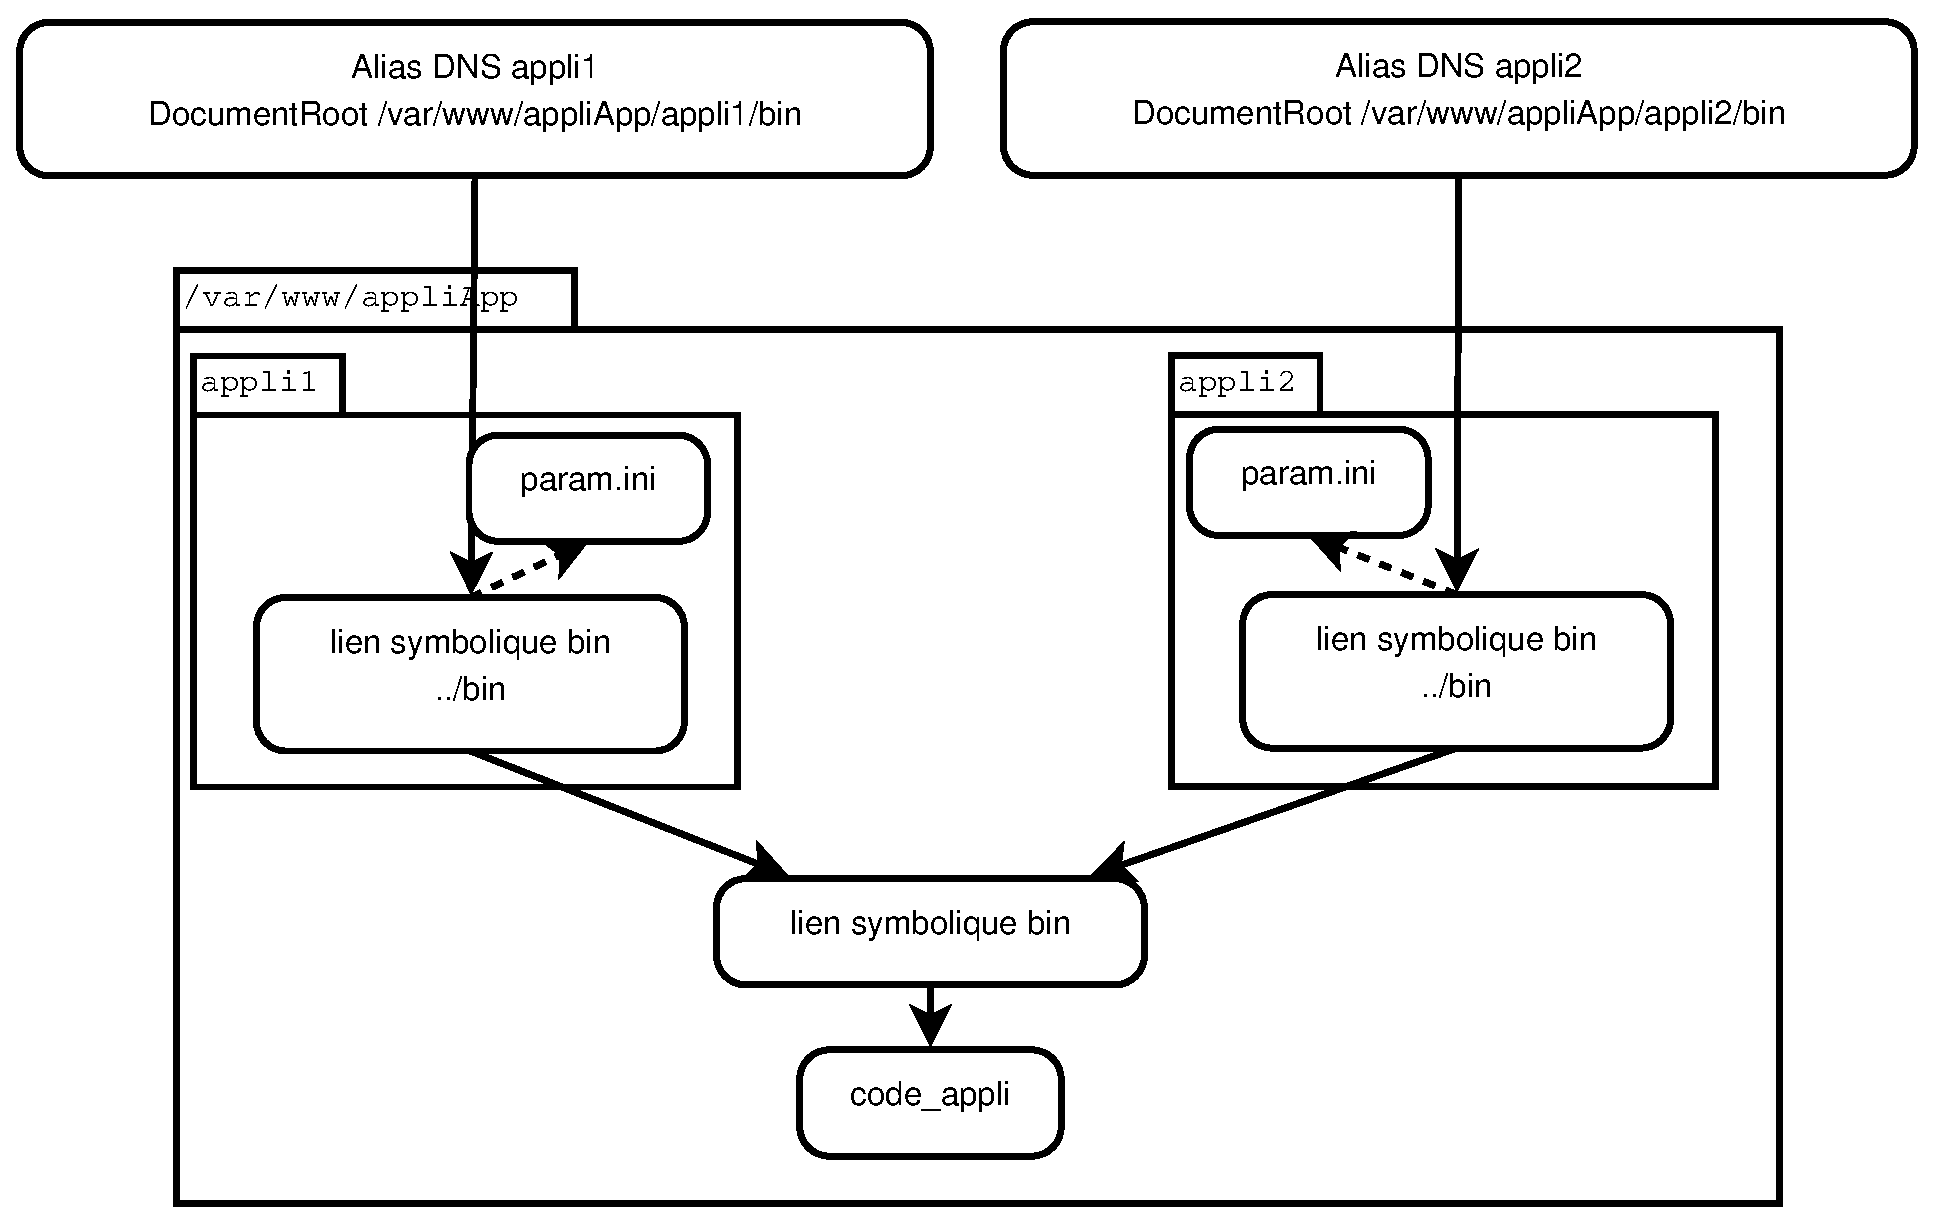
\includegraphics[width=\linewidth]{dessin/dnsmultiple}
\caption{Schéma général d'implémentation pour utiliser le même code avec des noms d'application et des jeux de données différents}
\end{figure}

Dans le paramétrage de l'alias DNS (en principe, dans \textbf{/etc/apache2/sites-available}), l'application pointe vers le dossier \textbf{/var/www/appliApp/appli1/bin}. 
\textit{/var/www} correspond à la racine du site web, \textit{appliApp} au dossier racine de l'application, \textit{appli1} au dossier spécifique de l'alias DNS.

Ce dossier \textit{appli1} ne contient que deux fichiers : \textbf{param.ini}, qui contient les paramètres spécifiques, et \textbf{bin}, qui est un lien symbolique vers le dossier \textbf{../bin}. 

Le dossier \textit{../bin} (donc, dans \textit{/var/www/appliApp}) est lui aussi un alias qui pointe vers le code réel de l'application, ici \textbf{code\_appli}.

Le fichier \textbf{param.inc.php} décrit l'entrée suivante :
\begin{lstlisting}
$paramIniFile = "../param.ini";
\end{lstlisting}

Le fichier \textbf{param.ini} sera cherché dans le dossier parent du code de l'application, c'est à dire soit dans \textit{appli1}, soit dans \textit{appli2} dans cet exemple.

Il suffit qu'il contienne les paramètres adéquats pour rendre l'application utilisable dans des contextes différents à partir du même code initial.